% LangClaw — JAIIO 2025/2026 submission (full paper, max 14 pages)
% Uses LNCS class (llncs.cls) as required by JAIIO guidelines.
% Anonymous submission: author/institute information omitted.
%
\documentclass{llncs}

\usepackage[a4paper, top=5.2cm, bottom=5.2cm, left=4.4cm, right=4.4cm]{geometry}
\usepackage[T1]{fontenc}
\usepackage[utf8]{inputenc}
\usepackage{mathptmx}
\usepackage{graphicx}
\usepackage{amsmath,amssymb}
\usepackage{booktabs}
\usepackage{algorithm}
\usepackage{algpseudocode}
\usepackage{listings}
\usepackage{enumitem}

\lstset{
  basicstyle=\small\ttfamily,
  breaklines=true,
  frame=single,
  language=Python,
  numbers=none,
  xleftmargin=1em,
  xrightmargin=1em,
}

\usepackage[style=apa]{biblatex}
\addbibresource{references.bib}

\begin{document}

% ============================================================
% ENGLISH TITLE + ABSTRACT + KEYWORDS
% ============================================================
\title{LangClaw: Endogenous Homeostatic Regulation for Mitigating Context
Collapse in Multi-Agent LLM Debate Systems}

% Anonymous submission — authors omitted for review
\author{}
\institute{}

\maketitle

\begin{abstract}
Multi-agent LLM systems tend to lose coherence as interaction extends---a
problem we term \emph{context collapse}. Existing frameworks address this
through static orchestration or periodic heartbeats, but both treat
participation frequency as a design constant. We ask whether it can instead
be an emergent property of each agent's internal regulatory state.
We present LangClaw, a framework grounded in a formal theory of homeostatic
agency in which each agent maintains an epistemic deficit
$\delta_i \in [\varepsilon,\infty)$ governed by a drive function
$D(\delta) = (\delta - \varepsilon)^2$; reward is defined as drive reduction,
implementing the equivalence theorem of Keramati and Gutkin (2014). A
multi-criteria stimulus evaluator acts as sensor; an online Q-learner
with $\varepsilon$-greedy exploration selects actions via TD(0). This
represents a structural departure from the prevailing heartbeat paradigm:
rather than firing on a fixed schedule, agents activate when internal
pressure warrants it and learn which actions most effectively reduce drive.
We evaluate LangClaw against a LangGraph-style LLM router under equal
heartbeat budgets in a zero-sum political debate with ten GPT-5-nano agents
organized as two VSM-inspired factions, measuring discourse structure through
AAF metrics, graph-structural peer reference, and the quality proxy
$\Delta\varphi^*$.

\keywords{multi-agent systems \and large language models \and homeostasis \and
reinforcement learning \and context collapse \and event-driven architecture}
\end{abstract}

% ============================================================
% SPANISH TITLE + RESUMEN + KEYWORDS
% ============================================================
\begin{center}
\vspace{1cm}
{\Large \bfseries\boldmath LangClaw: Regulaci\'on Homeost\'atica End\'ogena
para Mitigar el Colapso del Contexto en Sistemas de Debate Multi-Agente
basados en LLM}
\vspace{0.5cm}
\end{center}

\begin{abstract}
Los sistemas multi-agente LLM tienden a perder coherencia a medida que la
interacci\'on se extiende---un problema que denominamos \emph{colapso del
contexto}. Los frameworks existentes lo abordan mediante orquestaci\'on
est\'atica o heartbeats peri\'odicos, tratando la frecuencia de
participaci\'on como una constante de dise\~no. Presentamos LangClaw, un
framework donde cada agente mantiene un d\'eficit epist\'emico interno
$\delta_i \in [\varepsilon,\infty)$ gobernado por $D(\delta)=(\delta-\varepsilon)^2$;
la recompensa es reducci\'on de impulso $r_t = D(\delta_t)-D(\delta_{t+1})$
(teorema de Keramati y Gutkin, 2014). Un evaluador multicriterio act\'ua
como sensor; un Q-learner con pol\'itica $\varepsilon$-greedy selecciona
acciones via TD(0). Evaluamos LangClaw contra un enrutador al estilo LangGraph
en un debate pol\'itico con diez agentes GPT-5-nano organizados como dos
facciones VSM, midiendo coherencia argumentativa mediante m\'etricas AAF,
PRR$_G$ y $\Delta\varphi^*$.

\keywords{sistemas multi-agente \and modelos de lenguaje \and homeostasis \and
aprendizaje por refuerzo \and colapso del contexto \and arquitectura dirigida
por eventos}
\end{abstract}

\vspace{0.5cm}
\setcounter{page}{1}

% ============================================================
\section{Introduction}
\label{sec:intro}

Multi-agent LLM systems are moving toward sustained, deliberative
interaction---domains such as policy analysis, scientific peer review, and
institutional decision support where coherence over time is socially
consequential~\parencite{wang2024survey}. Two developments make this tractable
now: structured output enforcement enables closed regulatory loops over LLM
agents (unreliable before 2024), and scaling laws for inference-time
compute~\parencite{snell2024scaling} raise a distributional question: given a
fixed budget, how should computation be allocated across agents?

Yet as interaction extends, the collective process tends to degrade. Agents
may lose track of prior claims, repeat points, or produce structurally
disconnected monologues~\parencite{park2023generative}---a class of failures
we term \emph{context collapse}. The problem has a sociological precedent:
Michels' iron law of oligarchy~\parencite{michels1911political} established
that centralized coordination in deliberative organizations systematically
concentrates influence among contextually salient contributors. The mechanism
is informational, not intentional, and may apply equally to AI routers.

The dominant response has been external control---fixed turn schedules,
centralized routers, heartbeat daemons~\parencite{openclaw2026heartbeat}.
These approaches share a structural assumption: the activation decision
remains exogenous. The heartbeat fires at a fixed interval regardless of
discourse intensity; the router selects agents regardless of their internal
readiness. External orchestration may thus address the symptom without
explaining why coherence degrades.

Homeostatic reinforcement learning (HRRL)~\parencite{keramati2014homeostatic}
offers a different principle: regulation emerges from internal variables
that accumulate, trigger action, and return to equilibrium---no external
controller required. We propose LangClaw, in which each agent carries an
\emph{epistemic deficit} that grows when idle and shrinks after a
structurally useful contribution. A sigmoid gate maps deficit to action
probability; an online Q-learner selects actions and learns from drive
reduction. To our knowledge, this paradigm has not been evaluated as an
orchestration principle for LLM-based debate agents.

This paper makes three contributions: (1)~a formal theory of homeostatic
agency grounded in systemic materialism, allostatic regulation, and
eudaimonic motivation---making autonomy, drive, and quality-gated discharge
falsifiable rather than informal; (2)~an endogenous activation paradigm in
which participation frequency is an emergent property of internal
regulatory state, replacing the heartbeat/scheduler model; and (3)~an
experimental evaluation of whether neutral AI routers tend to replicate the
Michels dynamic---concentrating turns on the contextually dominant
faction---and whether homeostatic regulation counters this tendency.


% ============================================================
\section{Literature Review}
\label{sec:related}

Frameworks such as AutoGen~\parencite{wu2023autogen},
CAMEL~\parencite{li2023camel}, and MetaGPT~\parencite{hong2023metagpt}
demonstrate that role-specialized LLM collectives can coordinate on complex
tasks, but rely on predefined turn structures or centralized controllers---
\emph{externally organized} cooperation. The heartbeat
architecture~\parencite{openclaw2026heartbeat} adds temporal persistence, and
LangGraph provides durable state and workflow control, yet both still place
the activation decision outside the agent.
\textcite{huang2024masresilience} show that organizational form affects
resilience, with centralized structures degrading faster under stress.

Homeostatic reinforcement learning (HRRL)~\parencite{keramati2014homeostatic}
formalizes drive-reduction reward; continuous variants extend this to richer
dynamics~\parencite{laurencon2024ctcs}. Desire-driven LLM
agents~\parencite{wang2025d2a} treat internal variables as behavior-relevant
but do not close the loop through an explicit structural quality signal.
The gap is not whether LLM agents can have internal variables, but whether
those variables can govern activation and learning in a mathematically
explicit regulatory loop.

Our discourse model builds on Defeasible Logic
Programming~\parencite{simari1992mathematical,chesnevar2000logically,garcia2004defeasible}---a
tradition with foundational roots in Argentine AI---where claims are
defeasible and may be attacked by rebuttal or undercut. The adversarial
setting draws on the spirit of Sotopia~\parencite{zhou2024sotopia}, but our
focus is the structural evolution of argument graphs (defeat cycles,
acceptance dynamics, $\Delta\varphi^*$) rather than social realism.

% ============================================================
\section{Method}
\label{sec:method}

\subsection{A Theory of Homeostatic Agency}
\label{sec:theory}

Four postulates fix what autonomy requires, what triggers action, and what
makes an action valuable.  Every design choice below derives from them.

\subsubsection{Postulates.}

\noindent\textsc{P1} (Autonomy~\parencite{ashby1956introduction,beer1972brain}).
$a_i$ is \emph{autonomous} if its policy depends on internal state;
external schedulers collapse requisite variety to zero:
\begin{equation}
    \mathrm{Aut}(a_i) \;\iff\; \exists\,\delta_i \in S_L(a_i):\;
    \pi_i = \pi_i\!\bigl(\delta_i(t)\bigr)
    \label{eq:a1}
\end{equation}

\noindent\textsc{P2} (Drive~\parencite{sterling1988allostasis,friston2010free}).
Each $a_i$ has a drive $D$ zero at setpoint, increasing away from it;
activation probability is monotonically increasing in drive:
\begin{equation}
    D(\varepsilon)=0,\quad D'(\delta_i)>0 \;\forall\,\delta_i>\varepsilon,
    \quad p_i(t)=\sigma\!\bigl(D(\delta_i(t))\bigr)
    \label{eq:a2}
\end{equation}

\noindent\textsc{P3} (Quality-gating~\parencite{ryan2001happiness,huta2014eudaimonia}).
An isolated monologue modifies $V$ but not $\mathcal{S}_{\text{int}}$;
drive is reduced only by structurally integrated actions:
\begin{equation}
    g\!\bigl(\mathcal{S}(t),\mathcal{S}(t{+}1)\bigr)=0
    \;\Rightarrow\; \Delta\delta_i=0
    \label{eq:a3}
\end{equation}

\noindent\textsc{P4} (Measurability~\parencite{tononi2016integrated}).
Structural change is a computable function of the discourse graph;
with P3: $\Delta\delta_i = -\alpha\Delta_s$ when $\Delta_s>0$, else $0$:
\begin{equation}
    \Delta_s \;=\; g\!\bigl(\mathcal{S}(t),\mathcal{S}(t{+}1)\bigr),
    \quad g:\mathcal{S}\times\mathcal{S}\to\mathbb{R}_{\geq 0}
    \label{eq:a4}
\end{equation}

\noindent\textit{Predictions.} P1--P2: symmetric drive $\Rightarrow$ symmetric
activation (external routers lack this guarantee). P2--P4: bounded deficit
$\Rightarrow$ sustained participation, preventing unilateral silence.

\subsection{The Epistemic Drive}

P1--P4 state the requirements; the epistemic drive realizes them.
Each agent $i$ maintains epistemic deficit
$\delta_i \in [\varepsilon, \infty)$ with resting baseline
$\varepsilon = 0.1$, instantiating P2 and quality-coupled via P3,
grounded in HRRL~\parencite{keramati2014homeostatic}.
Five coupled mechanisms govern it.

\textbf{Decay.} At each heartbeat $t$:
\begin{equation}
    \delta_i^{(t+1)} = \delta_i^{(t)} + \lambda
    \label{eq:decay}
\end{equation}
with $\lambda = 0.05$, modeling the basal pressure to contribute.

\textbf{Sigmoid activation.} The probability of acting at heartbeat $t$:
\begin{equation}
    p_i^{(t)} = \frac{1}{1 + e^{-k(\delta_i^{(t)} - \theta)}}
    \label{eq:sigmoid}
\end{equation}
with $k = 10$, $\theta = 0.7$. Below $\theta$ the agent rests; above it,
the agent is compelled to participate.

\textbf{Stimulation.} A discourse event with relevance $r$ (Eq.~\ref{eq:stimulus})
pushes the deficit up:
\begin{equation}
    \delta_i^{(t+)} = \delta_i^{(t)} + \gamma \cdot r
    \label{eq:stimulate}
\end{equation}
with $\gamma = 0.1$. The deficit now integrates basal decay and discourse-driven
stimuli, making it a sensor of the agent's epistemic state relative to the
evolving debate.

\textbf{Satiation.} After producing an argument with quality $\Delta\varphi^*$:
\begin{equation}
    \delta_i^{\text{new}} = \max\!\bigl(\varepsilon,\;
        \delta_i - \alpha \cdot \Delta\varphi^*\bigr)
    \label{eq:satiation}
\end{equation}
where $\alpha$ is selected by the calibration procedure (Section~\ref{sec:setup}).
If $\Delta\varphi^* = 0$, the deficit does not decrease (P3): speaking without
engaging the discourse structure provides no regulatory relief.

\textbf{Drive function.} Following~\textcite{keramati2014homeostatic}:
\begin{equation}
    D(\delta_i) = (\delta_i - \varepsilon)^m, \quad m = 2
    \label{eq:drive}
\end{equation}
The quadratic form penalizes deviations from setpoint superlinearly, creating
stronger urgency to act as deficit grows.

\textbf{Homeostatic reward.} Reward is not an external signal but drive
reduction~\parencite{keramati2014homeostatic}:
\begin{equation}
    r_t = D(\delta_t) - D(\delta_{t+1})
    \label{eq:reward}
\end{equation}
By the equivalence theorem, a policy maximizing expected discounted reward
simultaneously minimizes expected future drive.

\textbf{Online Q-learning.} State features
$\phi(s) = [\delta,\; \delta^2,\; \rho_G,\; n_{\text{stim}}]$
(graph density $\rho_G$, buffered stimuli $n_{\text{stim}}$); linear
Q-function $Q(s,a) = \mathbf{w}_a^\top \phi(s)$; TD(0) update:
\begin{equation}
    \mathbf{w}_a \leftarrow \mathbf{w}_a + \eta \bigl[r + \gamma \max_{a'}
    Q(s', a') - Q(s, a)\bigr] \phi(s)
    \label{eq:td0}
\end{equation}
Weights are zero-initialized; action selection is $\varepsilon$-greedy
($\varepsilon=0.1$). Convergence within the horizon is not assumed; weights
are interpreted as adaptive control parameters, not a converged policy.

\subsection{Argument Graph and $\Phi^*$ Proxy}

P3--P4 demand a computable quality signal.  Surface metrics (BLEU, ROUGE,
BERTScore) capture fluency, not structural integration; we construct
$\Delta\varphi^*$ to operationalize structural engagement in the discourse
graph $G=(V,E)$, where nodes are defeasible
arguments~\parencite{garcia2004defeasible} and edges are attack relations.
When agent $i$ adds node $v$ attacking target $u$:

\begin{equation}
    \Delta\varphi^* = \tfrac{1}{3} C_B(u) + \tfrac{1}{3}
        \mathbb{1}_{\text{cycle}}(v,u) + \tfrac{1}{3} D(u)
    \label{eq:phi}
\end{equation}

where $C_B(u)$ is betweenness centrality (rewards engaging structurally
central claims), $\mathbb{1}_{\text{cycle}}$ indicates a new dialectical
cycle (A attacks B, B attacks C, C attacks A), and $D(u)$ is agent diversity
at the target (rewards entering contested territory). Equal weights reflect a
maximum-entropy prior. Isolated nodes get $\Delta\varphi^* = 0$. We use
$\Delta\varphi^*$ strictly as an operational structural measure, not as a
claim about information integration in the IIT sense.

\subsection{Action Space and Stimulus Evaluation}

Drive and quality signal require actions and a sensor linking discourse
events to internal state.  Each agent selects from five action types: \textbf{DEBATE} (produce an
argument, either stimulus-driven or proactive), \textbf{SEARCH} (acquire a
domain fact), \textbf{READ} (synthesize and consolidate recent graph state),
\textbf{MESSAGE} (send a directed communicative act to a specific allied
agent), or \textbf{PASS} (rest). This action set is identical in HRRL and
LangGraph; the difference between conditions lies in activation, not in local
capability.

Two subsystems govern action selection, each with a distinct role.

The \emph{StimulusEvaluator} acts as a \textbf{sensor}. When a
\texttt{NewArgumentEvent} arrives, it computes relevance across five
weighted criteria:

\begin{equation}
    U(\text{stimulus}) = w_F \cdot F + w_C \cdot C_B(u) + w_M \cdot M
        + w_N \cdot N + w_P \cdot P,
    \label{eq:stimulus}
\end{equation}
with $w_F + w_C + w_M + w_N + w_P = 1$.

\noindent where $F$ is faction relevance, $C_B(u)$ is betweenness
centrality of the attacked node, $M$ is strategic memory relevance, $N$ is
novelty (reduced if an ally already responded), and $P$ is unanswered
pressure. This relevance score feeds the \texttt{stimulate()} mechanism
(Eq.~\ref{eq:stimulate}), modulating the agent's deficit in response to
discourse events. The stimulus weights are not fixed ad hoc.  We begin from an
equal-importance prior and calibrate five alternative weight profiles by
micro-simulation before the main benchmark (Section~\ref{sec:setup}).
The calibration selected a \emph{faction-dominant} profile
($w_F{=}0.40$, remaining weights $0.15$ each), which prioritizes
faction relevance as a stimulus signal---consistent with the zero-sum
adversarial structure of the debate.

The \emph{Q-learner} acts as the \textbf{decision maker}: after the
sigmoid gate passes (Eq.~\ref{eq:sigmoid}), it selects an action via
$\varepsilon$-greedy ($\varepsilon=0.1$; Sutton \& Barto, 2018, \S2.3)
and updates weights from homeostatic reward (Eqs.~\ref{eq:reward},
\ref{eq:td0}), adapting preferences toward actions that most reduce drive.


\subsection{Three-Layer Memory}

Each agent maintains episodic, semantic, and working memory, all backed by
LangGraph's \texttt{InMemoryStore}.  Both conditions share identical memory
infrastructure, isolating the orchestration mechanism as the sole variable.

\subsection{Event-Driven Architecture}

Drive, quality signal, actions, sensor, and memory integrate into a single
event-driven cognitive loop.  Each agent is an event-processing entity following a
THINK--PLAN--EXECUTE--OBSERVE cognitive loop per heartbeat: buffered
\texttt{NewArgumentEvent}s are drained, $\delta_i$ incremented by decay,
the stimulus evaluator scores events (Eq.~\ref{eq:stimulus}), and the
sigmoid gate (Eq.~\ref{eq:sigmoid}) determines execution.  Satiation and
TD update close the loop (Eqs.~\ref{eq:satiation}, \ref{eq:td0}).
Figure~\ref{fig:agent_architecture} summarizes the architecture.

\begin{figure}[t]
    \centering
    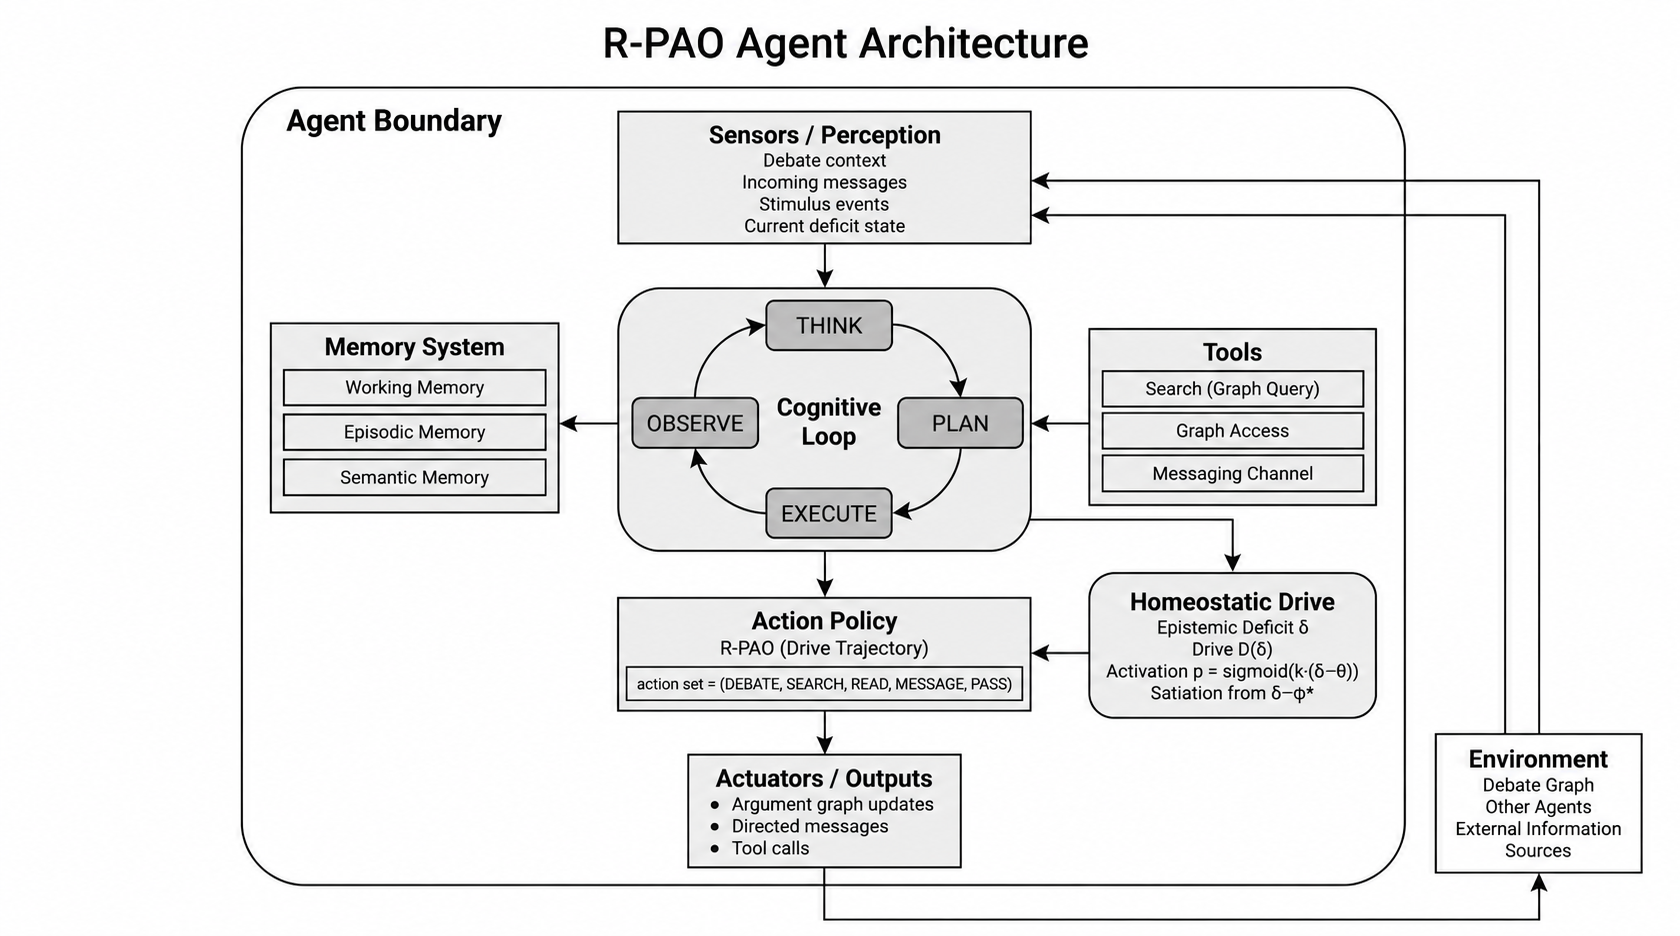
\includegraphics[width=0.92\linewidth]{langclaw/figs/illustration_1.png}
    \caption{LangClaw agent architecture: cognitive loop, memory, tools,
    and homeostatic drive.}
    \label{fig:agent_architecture}
\end{figure}

\subsection{Agent Roles: VSM-Inspired Faction Design}

From agent to system.  Both conditions share the same ten-agent
structure: two mirrored factions (Government/Opposition), each decomposed into five VSM
subsystems~\parencite{beer1972brain} (S1--S5).
Figure~\ref{fig:mas_vsm_architecture} shows the architecture.

\begin{figure}[t]
    \centering
    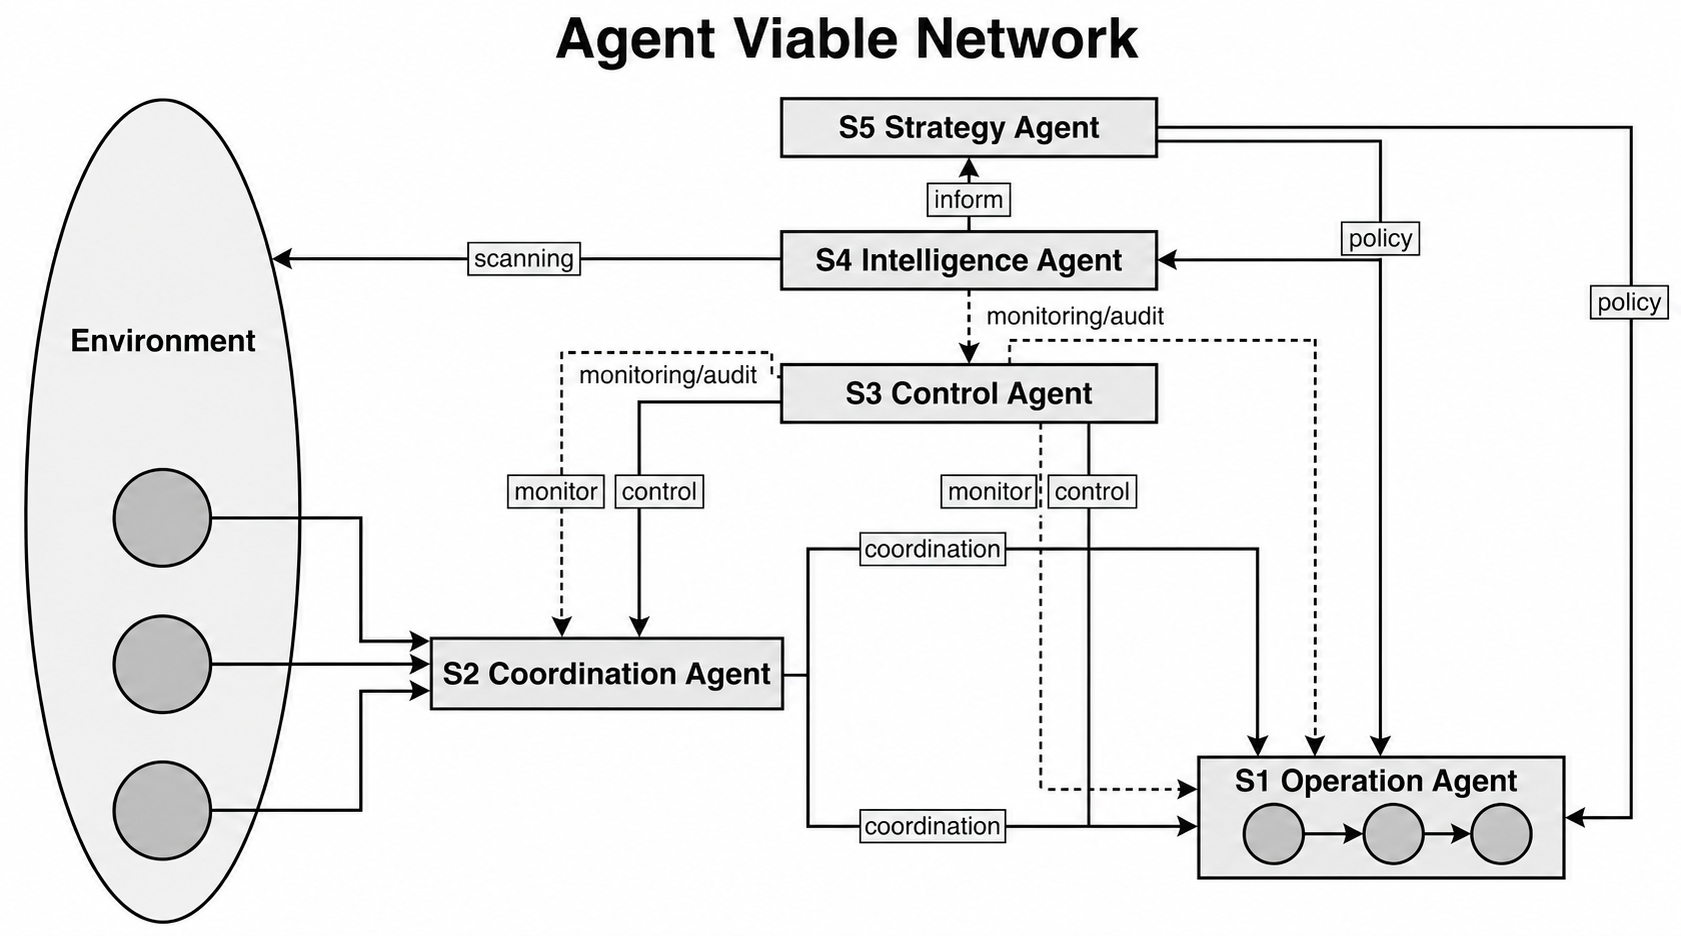
\includegraphics[width=0.95\linewidth]{langclaw/figs/illustration_2.png}
    \caption{VSM-inspired multi-agent architecture used in LangClaw: mirrored
    factional organization and shared discourse environment.}
    \label{fig:mas_vsm_architecture}
\end{figure}

\begin{table}
\caption{VSM subsystem roles (mirrored across both factions).}
\label{tab:roles}
\small
\begin{tabular}{|l|l|p{6cm}|}
\hline
\textbf{VSM} & \textbf{Role} & \textbf{Primary function} \\
\hline
S1 & Operations & Produce and defend claims; execute assigned debate tasks. \\
S2 & Coordination & Synchronize allied action; delegate tasks; route strategic information. \\
S3 & Control & Audit internal coherence; detect contradictions; send corrective messages. \\
S4 & Intelligence & Scan opponent; identify threats; use SEARCH for external resources. \\
S5 & Strategy & Set priorities; resolve control--intelligence tensions; issue directives. \\
\hline
\end{tabular}
\end{table}


\subsection{Orchestration Modes}

Agent and system defined, the experimental variable is isolated: who
decides when an agent acts.
We compare two conditions sharing the same memory, prompts, action space,
cognitive phases, and model backend.  In \textbf{HRRL} (endogenous), each
agent gates execution through its deficit-sigmoid
(Eq.~\ref{eq:sigmoid}) and selects actions via online Q-learning
(Eq.~\ref{eq:td0}) with homeostatic reward (Eq.~\ref{eq:reward}).
In \textbf{LangGraph} (exogenous baseline), a neutral LLM router reads the
discourse state and selects which agent enters the cognitive loop; the
selected agent then executes the same local capabilities.  The sole
difference is \emph{where} the activation decision is made.  Both run for
the same heartbeat horizon.

\subsection{Evaluation Metrics}

We use structural metrics over the argument graph rather than surface
fluency.  \textbf{AAF metrics}~(Dung, 1995): \emph{defeat cycle count}
$\lvert\text{SCC}_{>1}\rvert$ (mutual refutation cycles) and
\emph{acceptance ratio}
$\alpha = \lvert G \rvert / \lvert A \rvert$ (grounded extension over
total arguments; $\alpha{=}1$: all undefeated; $\alpha{=}0$: all
contested).  \textbf{PRR$_G$}: fraction of debates targeting an existing
node~\parencite{marandi2026prr}.  \textbf{$\Delta\varphi^*$}
(Eq.~\ref{eq:phi}): structural engagement per intervention.
\textbf{IR} (manipulation check): ratio of homeostatic-triggered to
total active turns; IR${=}1.0$ for HRRL, ${=}0.0$ for LangGraph.

\subsubsection{Central Hypothesis.}

\emph{Under equal heartbeat budgets and identical local capabilities,
endogenous homeostatic regulation sustains autonomy and argumentative
coherence over time more robustly than exogenous routing.}  The primary
measure is temporal degradation---per-heartbeat trajectories of
$\Delta\varphi^*$ and acceptance ratio compared by slope;
final-snapshot values (Table~\ref{tab:results}) are secondary.


% ============================================================
\section{Experimental Setup}
\label{sec:setup}

\begin{table}
\caption{Hyperparameters.}\label{tab:hyperparams}
\small
\begin{tabular}{|l|l|l|}
\hline
\textbf{Parameter} & \textbf{Symbol} & \textbf{Value} \\
\hline
Decay rate & $\lambda$ & 0.05 \\
Sigmoid steepness & $k$ & 10 \\
Activation threshold & $\theta$ & 0.7 \\
Satiation rate & $\alpha$ & 3.0 (calibrated from $\{1,2,3\}$) \\
Stimulus gain & $\gamma$ & 0.1 \\
Baseline / initial deficit & $\varepsilon$, $\delta_0$ & 0.1, 0.5 \\
Drive exponent & $m$ & 2 \\
Q-learning rate & $\eta$ & 0.01 \\
Exploration rate & $\varepsilon_{\text{RL}}$ & 0.1 \\
Discount factor & $\gamma_{\text{RL}}$ & 0.95 \\
Stimulus weights & $(w_F,w_C,w_M,w_N,w_P)$ & $(0.40, 0.15, 0.15, 0.15, 0.15)$ \\
Max heartbeats / agents & $T$, $N$ & 80, 10 \\
LLM & --- & GPT-5-nano \\
Seeds & $s$ & $\{7,17,42,123,256\}$ \\
\hline
\end{tabular}
\end{table}

\noindent Theory-grounded parameters ($\theta$, $\lambda$, $k$, $\varepsilon$,
$m$, $\eta$, $\gamma_{\text{RL}}$) were fixed from the formal model or
standard RL practice (Sutton \& Barto, 2018); $\alpha$ and the
stimulus-weight profile were selected by a pre-benchmark calibration stage
described below.

\subsection{Calibration and Protocol}

Two parameters lack theoretical priors: the satiation rate $\alpha$ and the
stimulus-weight vector $(w_F, w_C, w_M, w_N, w_P)$.  We calibrate them
empirically before the main benchmark to prevent arbitrary choices.

A 15-run micro-simulation ablation crosses five weight profiles---\emph{equal}
($1/5$ each), \emph{faction-dominant} ($w_F{=}0.40$, rest $0.15$),
\emph{centrality-dominant} ($w_C{=}0.40$), \emph{novelty-dominant}
($w_N{=}0.40$), and \emph{pressure-dominant} ($w_P{=}0.40$)---with three
$\alpha$ values ($\{1, 2, 3\}$).  Each micro-run executes 10 HRRL heartbeats
with seed $s{=}42$ and ranks configurations by mean
$\Delta\varphi^*$, with consistency as tiebreaker.
Table~\ref{tab:calibration} shows the top five results.

\begin{table}
\caption{Top-5 calibration results (10-heartbeat ablation, seed 42,
ranked by mean $\Delta\varphi^*$).}\label{tab:calibration}
\small
\begin{tabular}{|r|l|r|r|r|r|}
\hline
\textbf{Rank} & \textbf{Weight profile} & $\boldsymbol{\alpha}$ &
  \textbf{Debates} & $\overline{\Delta\varphi^*}$ &
  \textbf{Consist.} \\
\hline
1 & faction-dominant & 3.0 & 36 & 0.1356 & 97.2\% \\
2 & novelty-dominant & 1.0 & 30 & 0.1277 & 96.7\% \\
3 & faction-dominant & 2.0 & 31 & 0.1238 & 96.8\% \\
4 & equal            & 1.0 & 34 & 0.1210 & 97.1\% \\
5 & equal            & 3.0 & 38 & 0.1188 & 97.4\% \\
\hline
\end{tabular}
\end{table}

The winning configuration (\emph{faction-dominant}, $\alpha{=}3.0$) is frozen
for the full benchmark.  This result is interpretable: doubling the faction
weight makes the stimulus evaluator more responsive to attacks on in-group
claims, aligning the sensor with the zero-sum debate structure.  High
$\alpha$ amplifies satiation per unit of $\Delta\varphi^*$, encouraging the
agent to seek structurally impactful contributions rather than accumulating
low-quality debates.  The calibration was performed exclusively on HRRL;
LangGraph never sees these weights during tuning, preventing cross-condition
contamination.

Agent outputs enforce a Pydantic JSON schema; failed parses incur a
deficit penalty of $+0.1$ after two retries (equal to two decay steps,
penalizing structural failures proportionally to their temporal cost).
The benchmark script runs both modes for each seed sequentially.  A seed
factory derives deterministic prime seeds for each agent's RNG and LLM call
via SHA-256 hashing, ensuring reproducibility.  We run five seeds
($s \in \{7, 17, 42, 123, 256\}$) and report mean $\pm$ standard deviation.
Statistical tests use one-sided Welch's $t$-test with Bonferroni correction.

% ============================================================
\section{Results}
\label{sec:results}

\subsection{Outcome Metrics}

\begin{table}
\caption{Comparative results (mean $\pm$ std across 5 seeds, $T=80$
heartbeats). HRRL: online Q-learning with TD(0). LangGraph: exogenous
router, same temporal horizon.}\label{tab:results}
\begin{tabular}{|l|c|c|}
\hline
\textbf{Metric} & \textbf{HRRL} & \textbf{LangGraph} \\
\hline
Total debates              & 74.0 $\pm$ 9.6  & 74.0 $\pm$ 9.6 \\
Graph nodes                & 74.0 $\pm$ 9.6  & 74.0 $\pm$ 9.6 \\
Graph edges                & 72.8 $\pm$ 9.3  & 73.0 $\pm$ 9.6 \\
\hline
Per-agent $\sigma_s$ (\textbf{H}) & 1.53 $\pm$ 0.58 & 6.80 $\pm$ 1.14 \\
\hline
AAF defeat cycles          & 0 $\pm$ 0 & 0 $\pm$ 0 \\
AAF acceptance ratio       & 0.566 $\pm$ 0.021 & 0.711 $\pm$ 0.043 \\
PRR$_G$                    & 0.984 $\pm$ 0.004 & 0.986 $\pm$ 0.002 \\
Avg $\Delta\varphi^*$      & 0.149 $\pm$ 0.010 & 0.157 $\pm$ 0.011 \\
Avg reward (drive reduction) & 0.154 $\pm$ 0.015 & --- \\
\hline
IR (validity check)        & 1.0 & 0.0 \\
Stimulus-driven debates    & 63.6 $\pm$ 11.3 & --- \\
Avg stimulus utility       & 0.586 $\pm$ 0.031 & --- \\
\hline
\end{tabular}
\end{table}

IR = 1.0 for HRRL and 0.0 for LangGraph across all seeds (manipulation
check passed: modes are structurally distinct). Table~\ref{tab:results}
presents outcomes; five patterns stand out.

\textbf{H confirmed: balanced participation as emergent property.} HRRL
produces a mean per-seed per-agent standard deviation $\bar{\sigma}_s =
1.53 \pm 0.58$, compared to $6.80 \pm 1.14$ for LangGraph ($t = -8.1$,
$df = 5.9$, $p < 0.001$, $d = -5.1$). The effect is large and consistent
across all five seeds. HRRL distributes debates nearly uniformly
($\sim$18.4 per agent), whereas LangGraph's router exhibits systematic
bias toward opposition agents (OPP: $\sim$25 vs.\ GOV: $\sim$12). This
$2.1\times$ imbalance reflects the router's tendency to favor the
attacking faction --- an instance of the Michels dynamic, where the
coordinator's contextual-relevance heuristic amplifies the informational
advantage of the more salient faction.

\textbf{Comparable argument quality.} HRRL achieves $\Delta\varphi^* =
0.149 \pm 0.010$, comparable to LangGraph's $0.157 \pm 0.011$. LangGraph
achieves marginally higher per-intervention quality; this difference is
not statistically significant at $\alpha = 0.05$ but is directionally
consistent across seeds ($d = -0.84$). The data suggests that endogenous
regulation achieves near-equivalent quality to centralized routing without
the overhead of an external selection function.

\textbf{More contested discourse under HRRL.} HRRL produces a lower AAF
acceptance ratio (0.566 vs 0.711): more claims face counter-arguments
when all agents contribute equally. A lower $\alpha$ signals more
contested discourse, not inferior quality.

\textbf{Stimulus-driven behavior.} 86\% of HRRL debates (63.6/74.0) are
triggered by specific discourse events, consistent with genuine
stimulus-response behavior. The average drive-reduction reward is
$r = 0.154 \pm 0.015$, confirming DEBATE actions reduce epistemic drive
as predicted. Q-weight learning converges in direction: DEBATE\_STIMULUS
$= 0.247 \pm 0.076 >$ DEBATE\_PROACTIVE $= 0.186 \pm 0.044 >$ SEARCH $>$
READ, stable across all five seeds---consistent with the agent learning to
prioritize stimulus-responsive engagement over proactive exploration.

\subsection{Statistical Test}

\begin{table}
\caption{One-sided Welch's $t$-test ($n=5$ matched pairs) for H
(participation equity). Per-seed $\sigma_s$ = std.\ dev.\ of per-agent
debate counts within each seed.}\label{tab:stats}
\begin{tabular}{|l|c|c|c|c|}
\hline
\textbf{Hypothesis} & \textbf{$t$} & \textbf{$df$} & \textbf{$p$} &
\textbf{Cohen's $d$} \\
\hline
H: $\sigma_{\text{HRRL}} < \sigma_{\text{LG}}$ & $-8.1$ & 5.9 & $< 0.001$ & $-5.1$ \\
\hline
\end{tabular}
\end{table}

H is confirmed ($t = -8.1$, $d = -5.1$, $n=5$ exploratory; $n\geq 12$
needed for $d=0.5$ at 80\% power, though $d=-5.1$ is robust to seed
variation).


% ============================================================
\section{Discussion}
\label{sec:discussion}

\subsection{Interpreting the Results}

The data is consistent with H: HRRL sustains more balanced and contested
discourse dynamics than LangGraph under an equal temporal budget. The most
striking observation is participation balance ($\bar{\sigma}_s$: 1.53 vs
6.80, $p < 0.001$), consistent with symmetric drive mechanics preventing the
concentration of turns that Michels documented in deliberative
organizations---here replicated at the algorithmic level by exogenous
routing. This is an observation, not yet a confirmed causal claim; the
mechanism requires testing across longer horizons and varied configurations.

HRRL deficits oscillate around $\theta = 0.7$ (final means: 0.50--0.66)
through bootstrap, stimulus-onset, and homeostatic-oscillation phases.
LangGraph deficits grow monotonically (2.1--3.6), confirming the absence
of self-regulation. Argument quality is comparable across conditions
($d = -0.84$, n.s.), suggesting that endogenous regulation matches
centralized routing in per-intervention quality while distributing compute
more uniformly---a property that may become decisive under tighter budgets
or larger agent populations~\parencite{snell2024scaling}.

The absence of AAF defeat cycles in both modes reflects the debate's
asymmetric attack pattern (opposition attacks, government defends);
prompting strategies that encourage reciprocal counter-attack are future
work.

Two objections deserve direct response. First, does the deficit reduce to
a priority queue? A priority queue ranks but cannot adapt; the Q-learner
updates weights online from drive reduction, changing action preferences
over the course of the simulation. Second, does it resemble contextual
bandits? No: the deficit evolves endogenously through the drive function
(Eq.~\ref{eq:drive}) and reward depends on state transitions
(Eq.~\ref{eq:reward}), making this a sequential decision problem with
temporal discounting---not a stateless one.

A candid clarification: the regulatory \emph{mechanism} (deficit, threshold,
satiation parameters) was designed exogenously. What is endogenous is the
\emph{dynamics}: once in place, oscillatory equilibrium emerges from
agent--environment interaction without further external intervention.

\subsection{Limitations}

\begin{enumerate}
    \item \textbf{Statistical power}: $n=5$ seeds is exploratory; $n \geq 12$
          would be needed to detect $d = 0.5$ at 80\% power.
    \item \textbf{Q-learning convergence}: Weights are adaptive control
          parameters, not a converged policy within the 80-heartbeat horizon.
    \item \textbf{$\Phi^*$ proxy}: Equal weights are a principled prior;
          a learned or human-validated quality function remains future work.
    \item \textbf{LLM and scale}: Results are GPT-5-nano specific; longer
          horizons and larger populations remain to be tested.
    \item \textbf{Safety}: The deficit mechanism could be gamed by
          structurally well-placed but semantically vacuous arguments.
\end{enumerate}

\subsection{Further Research}

Key open directions: prompting strategies that induce reciprocal attack
(to make defeat cycles testable); hyperparameter sensitivity analysis for
$\theta$, $\alpha$, $\lambda$; scaling to larger populations and longer
horizons; replacing $\Delta\varphi^*$ with a learned quality function;
and evaluating HRRL under constrained inference-time compute budgets where
adaptive allocation may become a decisive advantage~\parencite{snell2024scaling}.

% ============================================================
\section{Conclusion}
\label{sec:conclusion}

LangClaw asks a concrete question: is context collapse in multi-agent LLM
debate better addressed through external scheduling or through endogenous
regulation? Preliminary results are consistent with endogenous regulation:
homeostatic mechanisms achieve comparable argument quality to LangGraph-style
routing while producing more balanced participation dynamics---an observation
consistent with the prediction that symmetric drive prevents the turn
concentration that neutral routers tend to produce.

The results do not establish which paradigm is universally superior, but
they show that endogenous regulation is competitive in quality while
producing structural properties---balanced participation, homeostatic
oscillation, stimulus-responsive activation---that centralized routing does
not produce by design in the present experiment.

% ============================================================
\section*{Reproducibility}

Complete code, seeds, and run instructions:
\url{https://github.com/pgerpe/langclaw_experiment}

% ============================================================
\begin{credits}
\subsubsection{\discintname}
The authors have no competing interests to declare that are relevant to the
content of this article.
\end{credits}

% ============================================================
\printbibliography

\end{document}
